\documentclass{book}
\usepackage{ctex}   % show Chinese
\usepackage{geometry}
\geometry{a4paper,centering,scale=0.8}
\usepackage{newtxtext}
\usepackage[dvipsnames,svgnames]{xcolor}
\usepackage{tcolorbox}
\usepackage[hidelinks]{hyperref}
\hypersetup{
  colorlinks,
  citecolor=violet,
  linkcolor=blue,
  urlcolor=blue}

% math 
\usepackage{amsmath}
\usepackage{amsfonts}
\usepackage{mathtools}

% insert code
\usepackage{listings}  
\definecolor{codegreen}{rgb}{0,0.6,0}
\definecolor{codegray}{rgb}{0.5,0.5,0.5}
\definecolor{codepurple}{rgb}{0.58,0,0.82}
\definecolor{backcolour}{rgb}{0.95,0.95,0.92}
\lstdefinestyle{mystyle}{
    backgroundcolor=\color{backcolour},   
    commentstyle=\color{codegreen},
    keywordstyle=\color{magenta},
    numberstyle=\tiny\color{codegray},
    stringstyle=\color{codepurple},
    basicstyle=\ttfamily\footnotesize,
    breakatwhitespace=false,         
    breaklines=true,                 
    captionpos=b,                    
    keepspaces=true,                 
    numbers=left,                    
    numbersep=5pt,                  
    showspaces=false,                
    showstringspaces=false,
    showtabs=false,                  
    tabsize=2
}
\lstset{style=mystyle}

% insert figures
\usepackage{graphicx}
\usepackage{subcaption}  % subfigure
\usepackage{caption}

% then can use \leqslant
\usepackage{amssymb}
% use this package to support & 
\usepackage{amsmath}


% use 4th order section
% https://tex.stackexchange.com/questions/427836/create-new-subsubsubsection-in-custom-class-file
\makeatletter
%same as \subsubsection but level 4
\renewcommand\paragraph{\@startsection{paragraph}{4}{\z@}%
                                     {-3.25ex\@plus -1ex \@minus -.2ex}%
                                     {1.5ex \@plus .2ex}%
                                     {\normalfont\normalsize\bfseries}}
% number \paragraph
\setcounter{secnumdepth}{4}

\makeatother








\title{title}
\author{author}

\includeonly{ch1}


\begin{document}

\maketitle

\tableofcontents
\newpage


\chapter{chapter 1}


\section{section1}
引用 \cite{tuszewski1988field}。

公式:
\begin{equation}
\bar{s} = \int_{r_o}^{r_s} \frac{r}{r_s \rho_i}   dr
\end{equation}

行内公式: $\bar{s}<2$, $r_o$。



itemize:
\begin{itemize}
\item item1
\item item2
\item item3
\end{itemize}

% 配色方案: https://zhuanlan.zhihu.com/p/336171630
% 以及: https://zhuanlan.zhihu.com/p/472540719
测试 box:
\begin{tcolorbox}
    [colback = Emerald!10, colframe = cyan!40!black, 
    title = title here]
    测试测试测试
\end{tcolorbox}


\begin{tcolorbox}[colback=OliveGreen!10,colframe=Green!70,
    title=title here]
    测试测试测试
    \begin{equation}
        a = \int \cos(x) dx
    \end{equation}
\end{tcolorbox}


\begin{tcolorbox}[colback=red!5,colframe=red!75!black,
    title = title here
    ]
    测试测试测试
\end{tcolorbox}

\begin{tcolorbox}
    [colback=Salmon!20, colframe=Salmon!90!Black,
    title = title here
    ]
    测试测试测试
\end{tcolorbox}

\begin{tcolorbox}
    [colback=Salmon!20, colframe=Salmon!90!Black
    ]
    测试没有title
\end{tcolorbox}



测试code:
\lstinputlisting[language=Python]{./example.py}


双图:
\begin{figure}[!hbtp]
    \centering
    \begin{subfigure}[b]{0.45\textwidth}
    \centering
    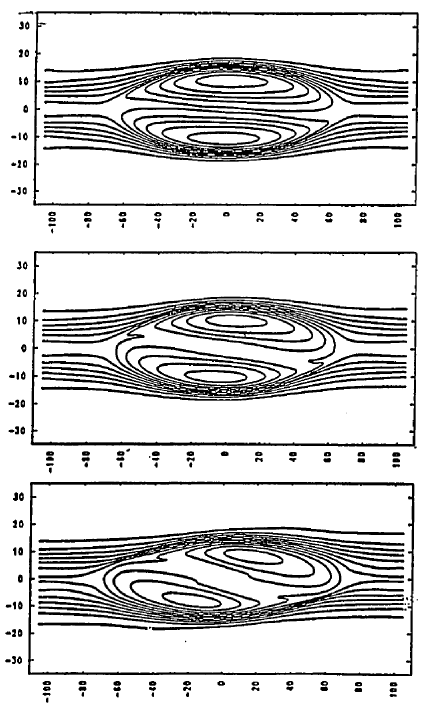
\includegraphics[width=0.9\textwidth]{figs/tilt.png} 
    \caption{evolution of density contours for the tilt mode}
    \label{fig: tilt}
    \end{subfigure}
    \hfill % this is very important!!!
    \begin{subfigure}[b]{0.45\textwidth}
    \centering
    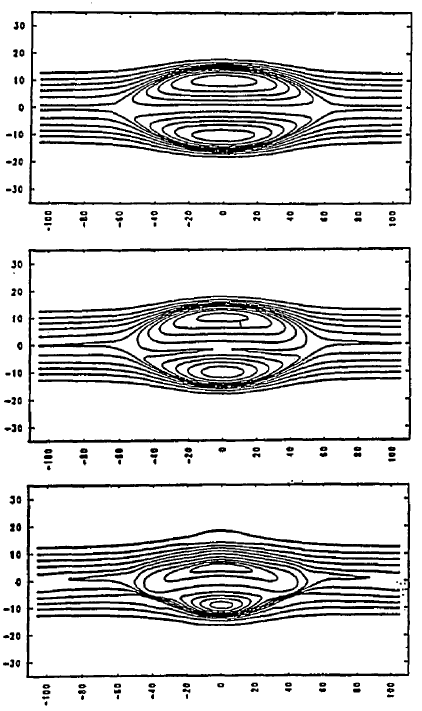
\includegraphics[width=0.9\textwidth]{figs/mushroom.png}
    \caption{evolution of density contours for the mushroom mode}
    \label{fig: mushroom}
    \end{subfigure}
    \caption{FRC中的倾斜模和蘑菇模\cite{staudenmeier1991fluid}}
    \label{fig: tilt and mushroom}
\end{figure}



\subsection{section 2}



\subsection{subsection}

词语带有网页链接, 比如: \href{https://zh.wikipedia.org/wiki/%E7%A3%81%E7%9F%A9}{磁力矩}。


插入单栏图片: 
\begin{figure}[!hbtp]
    \centering
    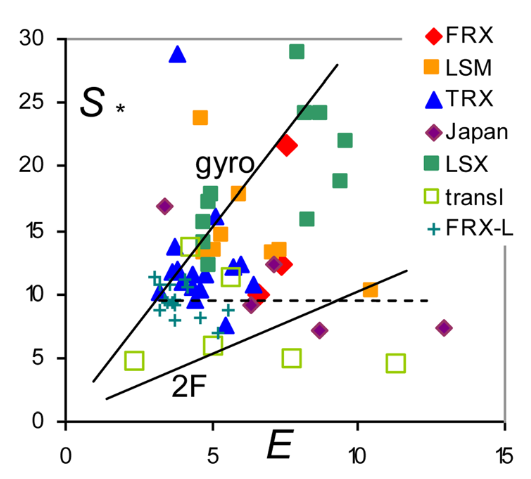
\includegraphics[width=0.5\textwidth]{figs/ctilt.png} 
    \caption{Size parameter vs separatrix elongation for elongated FRCs\cite{steinhauer2011review}}
    \label{fig: cgyro}
\end{figure}

插入表格: 
\begin{table}[!hbtp]
    \centering
    \begin{tabular}{lllll}
    \hline
    type & 1 & 2 & 3 & 4 \\ \hline
    1    & 2 & 3 & 4 & 5 \\ \hline
    1    & 2 & 3 & 4 & 5 \\ \hline
    1    & 2 & 3 & 4 & 5 \\ \hline
    \end{tabular}
\end{table}


% 参考文献
\bibliographystyle{IEEEtran}
\bibliography{references}






\end{document}
